\documentclass[a4paper,12pt,titlepage]{scrartcl}
\usepackage{graphicx}
\usepackage{url}
\usepackage{subcaption}
\usepackage{wrapfig}


\titlehead{
	\centering
	
\includegraphics[width=5in]{images/d3b.png}
	
\includegraphics[width=5in]{images/kidsfirst.png}
}
\title{Developer Handbook}
\date{\today}

\begin{document}

	\maketitle
	
	\tableofcontents
	\newpage
   
	\section{Welcome}
   
 	\section{Issues}
 	
 	Github Issues are used to maintain a backlog of work to be done for each repository as well as estimate and schedule work using Zenhub.
 	
	\subsection{Creating Issues}
	
	Issues may be created by users or internal developers for a handful of reasons from questions to feature requests to bugs.
	Creation of an issue should ideally happen the moment a bug is found or a new feature is desired to promote a shared awareness of that issue and provide a place to track it.
	Although Zenhub provides an overview of all issues in the organization, issues inherently belong to only one repository.
	When creating an issue, it is best to target and phrase it towards a single repository.
	If an issue seemingly spans many repositories, it likely needs to be broken down into more precise tasks.
	
	Issue labels (See section \ref{labels}) should be chosen as needed to easily sort through the backlog.
	Assigners should be appointed to an issue once they have volunteered to address the issue, or, at the latest, have begun work on it.
	There currently is no standard across D3b for formatting an issue body and should be implemented on a repository level.
	If a repository has an {\em Issue Template}, make sure to follow it!
      
	\subsection{Finding Issues}
	
	\subsection{Labels}\label{labels}
	
	Repositories across the D3b Github organization that have frequent user feedback and bug reports should use our standard set of labels to tag issues shown in Figure \ref{fig:labels}.
	Labels act as a means of filtering categories of issues and providing summaries of effort completed in release notes.
	Users that are not part of the organization may not add labels themselves, so please add labels as you see necessary to new issues.
	The {\b help wanted} label is a special label that is displayed in repository summaries on Github (See the {\em 11 Issues need help} in Figure \ref{fig:reposummary}).
	Use it to mark issues that are self-contained and do not require in-depth knowledge of how the code base works.
	This tag is useful for guiding new members or external contributors looking to get involved to issues that will be easy for them to accomplish.
   
  	\begin{figure}[h]
  			\centering
    			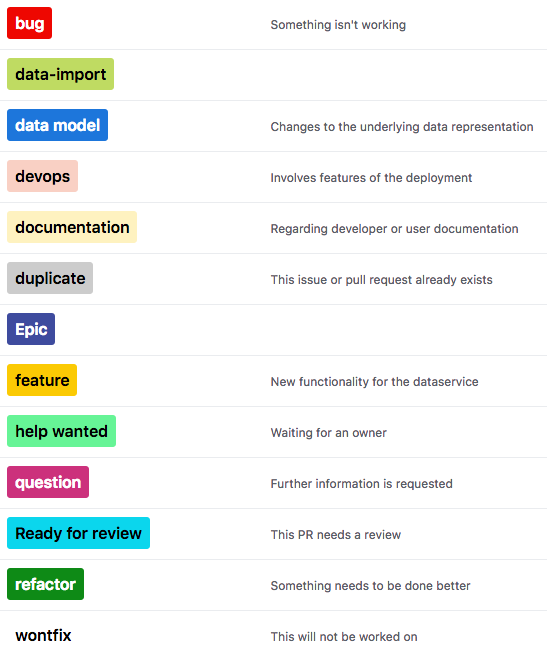
\includegraphics[width=0.4\textwidth]{images/labels.png}
    			\caption{Standard Repository labels with descriptions and colors}
    			\label{fig:labels}
   	\end{figure}
   
	\section{Creating a Pull Request}
	
	Creating a pull request is the first step to getting new code merged back into the code base.
	Opening of a new pull request may signify that changes are ready for review, or that the author wishes to give visibility into their current status.
	This section outlines the common standards and practices around the pull request and review process.
	
	\subsection{Commit Messages}\label{commits}
	
	\begin{figure}
	\centering
   	\begin{subfigure}[h]{0.4\textwidth}
    		\centering
    		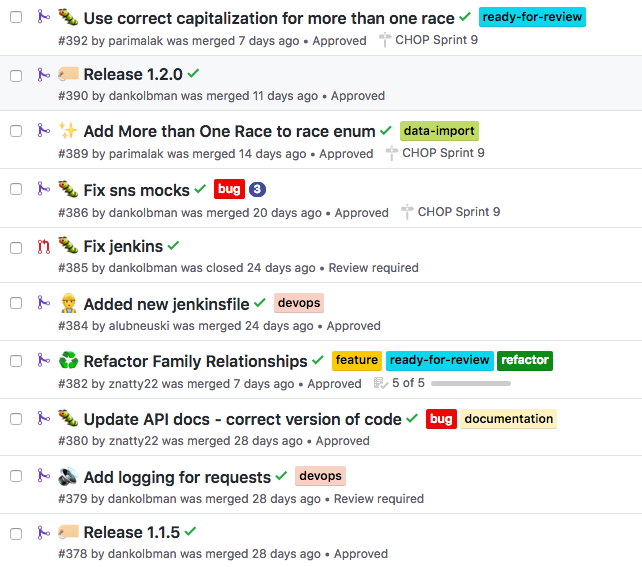
\includegraphics[width=\textwidth]{images/prhistory.png}
    		\caption{Closed pull requests in Github}
    		\label{fig:prhistory}
    	\end{subfigure}
    	 \hfill
  	\begin{subfigure}[h]{0.4\textwidth}
    		\centering
    		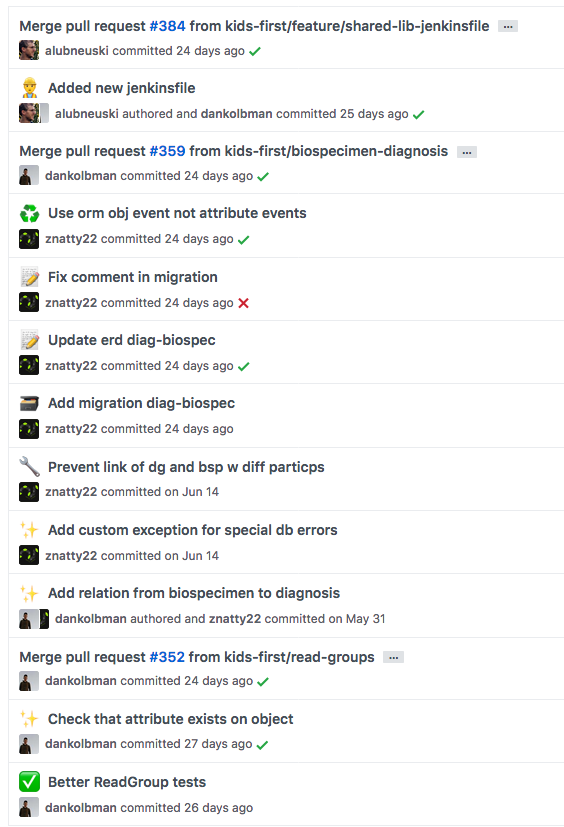
\includegraphics[width=\textwidth]{images/commithistory.png}
    		\caption{A slice of the dataservice commit history in Github.}
    		\label{fig:commithistory}
    	\end{subfigure}
    	\caption{Use of emojis in the dataservice.}
   	\end{figure}	
	
	Commit messages are vital in being able to navigate a code base's history.
	There are many resources providing best practices for commit messages \cite{beams, socommits}.
	
	We require commits to be prefixed with a single emoji that appropriately summarizes the the gist of the commit.
	This is helpful in allowing one to scan through the commit log visually inside of Github (Figure \ref{fig:commithistory}) or be able to perform summary analysis inside of release notes or when analyzing git activity as a whole.
	When adding an emoji to the commit message, use the colon-ated version as opposed to the actual unicode symbol, eg: {\em :sparkles:}.
	For inspiration of what emoji may be most appropriate, see the gitmoji guide \cite{gitmoji}.
	
	\subsection{Pull Request Titles}
	
	Pull request titles should begin with an emoji, similar to commit messages.
	This provides similar benefits to commit message emojis where past pull requests may quickly be scanned and summarized (Figure \ref{fig:prhistory}).
	
	\subsection{Keeping the Commit Log Tidy}
	
	In addition to best practices outlined in Section \ref{commits}, care should be taken to avoid introducing unhelpful commits such as merges of master into a feature branch.
	Often, a feature branch will become stale during development as other features are merged into master.
	Instead of using the {\em Update} button in Github to merge the latest master into the feature branch, one should opt to rebase the branch on the latest master.
	This will avoid adding many {\em Merged branch master} commits into a feature branches 
	
	\subsection{Labeling Pull Requests}
	
	The labels on pull requests are shared with those in issues (Section \ref{labels}, Figure \ref{fig:labels}).
	Pull requests should be labeled appropriately so that they may be filtered and analyzed easily.
	
	One special label that applies only to pull requests is the {\em ready-for-review} label.
	Marking an open pull request with this label signals to other developers that it is ready for a code review.
	This label may also be used by automated tooling to send notifications on un-reviewed pull requests
	
	\subsection{Requesting Reviews}
   	
   	Reviewers may be requested in Github inside of a pull request (Figure \ref{fig:requestreviewer}).
   	This will notify the user via Github notifications and email, if the user has them enabled.
   	Github notifications can be easily missed, so it is advised to use direct messing in Slack if the request is urgent.
   	
   	\begin{wrapfigure}{r}{0.3\textwidth}
  		\centering
    		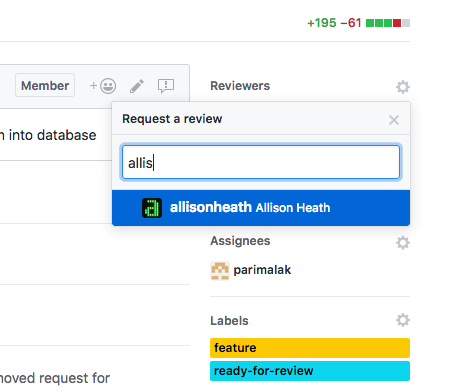
\includegraphics[width=0.4\textwidth]{images/requestreviewer.png}
    		\caption{Requesting a reviewer on a pull request.}
    		\label{fig:requestreviewer}
   	\end{wrapfigure}
   
	\section{Review Process}
	
	\subsection{Code Review}
	
	\subsection{Testing}
	
	Commit hooks should trigger testing integrations upon any push to master or a branch with an open pull request, at the least.
	Among these integrations should be at least on test runner that will run the repositories unit tests and report status back to Github.
	Having tests is critical to ensuring that new features are hardened for future development.
	Tests for new features in a pull request are expected to have tests included at the time of review.
	Existence and functionality of these tests should be checked as part of the review process.
	
	\subsection{Status Checks}
	
	Status checks is a feature in Github that listens to services that run in response to git hooks (Figure \ref{fig:statuschecks}).
	Pull requests will be prevented from merging until each of these services reports back positively on the state of the code.
	In addition to services, reviews are may also be included as status checks, requiring one or more approvals from reviewers before being marked as ok.
   
   	\begin{wrapfigure}{r}{0.4\textwidth}
  		\centering
    		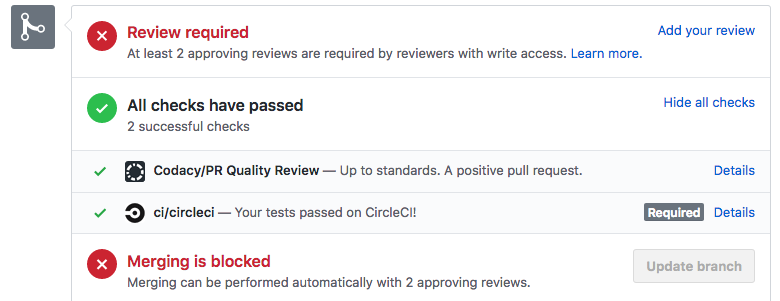
\includegraphics[width=0.4\textwidth]{images/statuschecks.png}
    		\caption{Status checks on a pull request.}
    		\label{fig:statuschecks}
   	\end{wrapfigure}
   	
   	\pagebreak
   	
	\section{Software Release}
	
	\section{New Repositories}
	
	\subsection{Naming}
	
	\subsection{Description}
	
	\subsection{Tags}
	
	\subsection{Protected Branches}
	
	\subsection{README}
	
	\subsection{License}
	
	Kids First uses the Apache 2.0 \cite{apache2} license exclusively for all public repositories.
	The file should be placed in the root of the directory with the name {\em LICENSE}.
	The Apache 2.0 license may be easily added from the root repository view on Github using {\em add new file} and naming it LICENSE.
	This will present a {\em Choose license template} button to the right of the file name where the Apache 2.0 License may be chosen to automatically populate the file (See Fig \ref{fig:addlicense}).
	
	\begin{figure}[t]
    		\centering
    		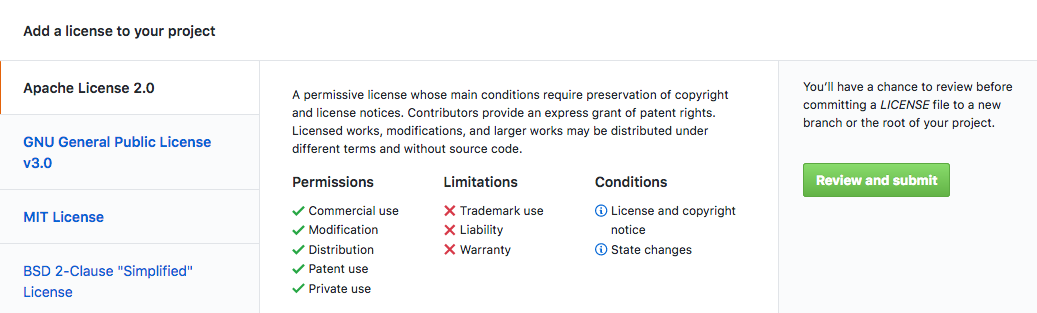
\includegraphics[width=0.8\linewidth]{images/license.png}
    		\caption{The Apache 2.0 license is available by default from the Github web interface.}
    		\label{fig:addlicense}
    \end{figure}
	
	\subsection{Config Repository}
	
	In addition to creating the main code repository, each code repository that is to be deployed must have a second, {\em private} repository that contains the infrastructure and CI/CD strategy for that code base.
	The repository for the config {\em must match the name of the code repository suffixed with -config}.
	This is a rule of thumb that is followed throughout so that the configuration may be discovered automatically by other scripts.
	In addition to the naming standard, the repository should be {\em private}.
	It is best practice to keep the infrastructure obscured and prevent external contributions as the config contains code that is often run at elevated privileges in our environments.
	
	\section{Environments}
	
	Often, entire software stacks are deployed concurrently in many different {\em environments}. This provides us with a handful of benefits:
	
	\begin{itemize}  
	\item Assurance that there is always a stable deployment for end-users
	\item Provides a safe sandbox to develop new features in isolation
	\item Insures the boilerplate to re-deploy a new environment exists
	\end{itemize}
	
	We divide our environments into three primary stages that are tightly couple to our Continuous Integration
	
	\subsection{dev}
	
	The development environment (dev) is intended as sandbox for  new features and code bases.
	It is the most unstable environment with no guarantees on data availability.
	When new code is pushed to a feature branch, it automatically triggers its CI pipeline to test, build, and, deploy to the development environment.
	The branch must pass through testing and deployment successfully to before it is allowed to be merged to insure that it will successfully deploy to the next stage.
	
	\subsection{qa}
	
	The QA environment provides a mostly-stable environment where new features may be used, evaluated, and tested before being released.
	This is is where integration test-suites may be run to ensure that all services cooperate nicely.
	The data in QA should also be close to production quality to fully flex all features.
	New features enter QA after merging a feature branch into the master branch of a code base.
	
	\subsection{prd}
	
	The production environment (prd) is the end-user environment.
	This is critically stable as it must be exposed to the public.
	To introduce features into prd, a repository must go through the release process.
	This includes creating a pull request for the version change, signoff on it from any potential stakeholders, merging, and finally acquiring final approval from an administrator to deploy the infrastructure and code into the environment.
	
	\begin{figure}
    		\centering
    		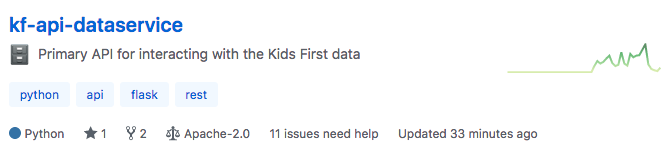
\includegraphics[width=0.6\linewidth]{images/reposummary.png}
    		\caption{An exemplary repository summary including: proper naming scheme, emoji followed by short description, labels, the {\em Apache 2.0} license, and issues tagged with {\em help wanted}}
    		\label{fig:reposummary}
    \end{figure}

	\bibliographystyle{plain}
	\bibliography{bibliography} 
\end{document}